\documentclass[12pt,a4paper]{report}
\usepackage[utf8]{inputenc}
\usepackage{amsmath}
\usepackage{amsfonts}
\usepackage{amssymb}
\usepackage{graphicx}
\usepackage{titlepic}
\usepackage{hyperref}
\usepackage{subfig}
\usepackage{svg}
\usepackage{float}
\usepackage[utf8]{inputenc}
\usepackage[left=2cm,right=2cm,top=2cm,bottom=2cm]{geometry}
\renewcommand{\thesection}{\arabic{section}}
\author{Braydan Newman - n11272031}
\title{
	Interactive Exploration of Fractal Geometry \\
	\large Case Study Final Report MXB362
	\footnotetext{All Fractal images are generated using "https://fractals.braydannewman.com/", unless specified otherwise}
}

\titlepic{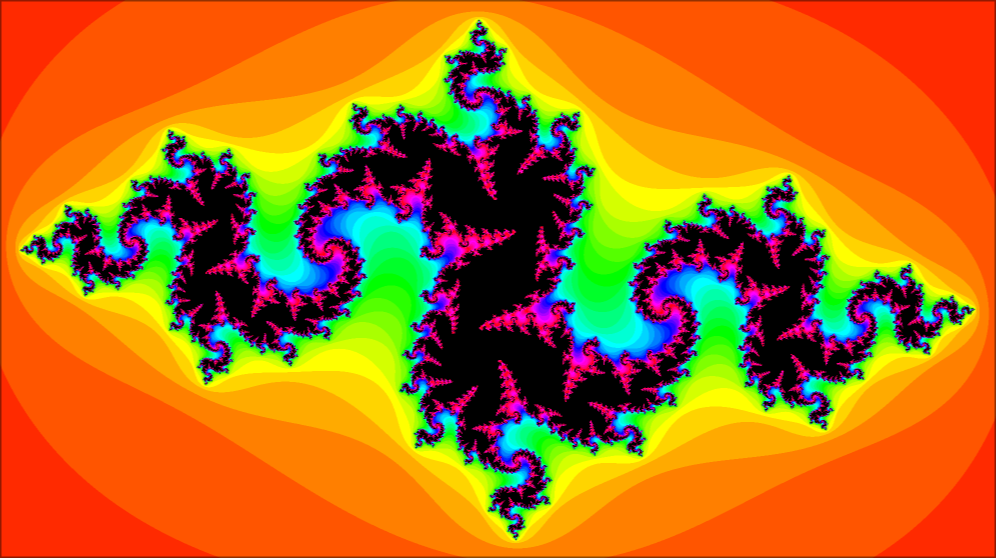
\includegraphics[width=\textwidth]{images/julia1.png}}
\begin{document}
\maketitle
\tableofcontents
\newpage

\section{Executive Summary}

The project aims to reimagine the exploration of fractal geometry by creating an interactive, web-based visualisation that links the Mandelbrot and Julia sets in real-time. This dynamic interface allows users to see how selecting any point within the Mandelbrot set directly influences the structure and connectiveness of the Julia set, with visually rich displays that highlight the inherent stability or chaos. Departing from static representations, the project empowers users to experience the relationship between these fractals through interactive features like an “infinite” scroll for in-depth zooming and real-time rendering of fractal changes.
\\\\
Key data in this project originates from complex number-based calculations used to generate both fractals. The Mandelbrot and Julia sets are created through iterative functions that test if values remain bounded. These calculations yield rich datasets, where each pixel’s colour maps to how rapidly the function diverges, creating visually intricate boundaries that depict fractal stability. The project is implemented using WebGL for rendering, which accelerates complex calculations, and JavaScript to handle user interaction, enabling responsive exploration. 
\\\\
The project's Visualisations integrate gradient colouring, hue-mapping, and smooth shading to make fractal boundaries vivid and continuous. Real-time interaction and zooming functions allow users to explore deeper layers within fractals, continuously recalculated with high resolution to reveal patterns at increasing magnifications. These features showcase fractal geometry’s recursive nature and deliver an engaging tool for visualising mathematical relationships. 
\\\\
In terms of novel contributions, this project incorporates a real-time Julia set generator, responsive to user-selected Mandelbrot coordinates, and implements an adaptive resolution zoom to manage performance, maintaining visual sharpness while users delve infinitely into the fractal’s depths. The results demonstrate how interactive tools can transform the way users learn and engage with complex mathematical concepts, making fractal geometry more accessible and captivating. 

\section{Description of the Project}
\subsection{Data Sources}
The project visualises two primary fractal structures: the Mandelbrot set and the Julia set. Both fractals are topological in nature, defined by their boundaries on the complex plane and the infinite detail within those boundaries. The Mandelbrot set data is generated by iterating a complex quadratic polynomial, where each point (pixel) on the complex plane corresponds to a complex number. If the function iteratively applied to this number does not diverge to infinity, the point is considered within the Mandelbrot set. In contrast, points that diverge are assigned colours based on the number of iterations needed to exceed a specified bound. 
\\\\
Similarly, the Julia set is generated using the same iterative approach, but with a constant complex parameter, c, derived from any selected point in the Mandelbrot set. The Julia set is essentially a unique fractal shape for every possible value of c. Each Julia set created reflects the characteristics of the Mandelbrot point chosen, producing connected and stable structures for points within the Mandelbrot set and fragmented, chaotic forms for points outside. 
\\\\
Data Visualisation of these fractals requires mapping complex numbers onto pixel grids, where colour gradients represent the escape time for each point. This colour mapping reveals fractal boundaries and produces vibrant, intricate patterns around stable and chaotic regions. Due to the fractals’ infinitely detailed structures, the Visualisation algorithm incorporates zoom features to display deeper layers of the fractal at higher resolutions. This requires dynamic recalculations and adaptive resolution to maintain image quality while managing performance. 

\subsection{Visualisation Techniques}
Several Visualisation techniques are used in the project to bring out the complex patterns within the Mandelbrot and Julia sets. Each technique supports interactive exploration by visually differentiating regions based on escape time and rendering the fractals in real time as users adjust parameters.

\paragraph{Colour Mapping and Gradient Shading}
Colour mapping translates the number of iterations needed for divergence into colour gradients, providing users with an intuitive view of fractal boundaries. Bound points are coloured in solid shades, while divergent points receive colours representing escape rates. Smooth gradient shading is applied to these colours, interpolating between hues to reduce visual noise and create continuity across complex edges. 

\paragraph{Hue-Based Colouring} 
To highlight fractal structure and make boundaries between stability and chaos more distinct, hue-based colouring is applied. Here, warm colours (e.g., reds, yellows) indicate rapid divergence, while cool colours (e.g., blues, greens) represent slower rates. This distinction enhances user understanding by making different behaviours within the fractals easily identifiable at various zoom levels. 

\paragraph{Real-Time Julia Set Generation} 
By linking user-selected points in the Mandelbrot set to Julia set calculations, the project dynamically generates a corresponding Julia set based on any complex value. This interaction updates the Julia set instantaneously as users hover or click on points in the Mandelbrot set, providing immediate visual feedback on the relationship between the two fractals. 

\paragraph{Infinite Zoom with Adaptive Resolution}
An “infinite” zoom feature enables users to delve into fractal structures at progressively finer resolutions. Adaptive resolution techniques maintain image sharpness by dynamically recalculating fractal data for deeper zoom levels. This technique avoids unnecessary computations for distant views, focusing processing power on detailed views at closer zooms. 

\subsection{Visualisation Environments and Tools}
The production of this project’s Visualisations involved several environments and tools that provided the necessary rendering power, interactivity management, and computational efficiency. 

\paragraph{WebGL (Graphics Environment)}
WebGL was the primary graphics environment used for rendering the Mandelbrot and Julia sets in real-time. Its support for GPU acceleration was essential, enabling complex iterative computations to be processed independently for each pixel. Fragment shaders in WebGL handled the calculations to determine if points escaped or remained bounded. Colour mappings were applied within the shaders to create smooth gradients, while WebGL’s parallel processing capabilities allowed the rendering of high-resolution fractals with minimal lag, even at deeper zoom levels. 

\paragraph{JavaScript (Development Environment)}
JavaScript served as the development environment for managing user interactions and passing user inputs to the WebGL shaders. It handled real-time events, such as mouse movements and clicks, capturing the (x, y) coordinates selected on the Mandelbrot set and feeding these as parameters for Julia set generation. JavaScript also facilitated zoom and pan functionalities, dynamically adjusting the viewing parameters in WebGL to ensure seamless zoom transitions and recalculations at adaptive resolutions. 
\\\\
This combination of WebGL and JavaScript allowed the creation of a real-time, interactive Visualisation platform. By leveraging GPU processing in WebGL, managing interactivity with JavaScript, the project achieved high performance and visual appeal in fractal exploration, rendering complex structures intuitively accessible to users. 

\section{Results and Outputs}
\subsection{Background Research and Investigations}
The project began with an exploration of fractal geometry, particularly the theoretical and computational foundations of the Mandelbrot and Julia sets. Fractals have intrigued mathematicians and scientists for their capacity to describe complex, self-similar patterns found in nature. Understanding the intricate details of the Mandelbrot and Julia sets required a deep dive into fractal theory, the iterative algorithms underlying these sets, and the unique relationship between these two fractals. 

\subsubsection{Fractal Theory and Mathematical Foundations}
The Mandelbrot set, introduced by mathematician Benoît B. Mandelbrot in the 1980s, is derived from a quadratic function that iterates over complex numbers. A point $c$ on the complex plane is tested for whether it remains bounded or diverges to infinity under repeated iterations of the function 
$z_{n+1}=z_n^2 + c$. Points that remain bounded under a set iteration threshold are part of the Mandelbrot set, while those that diverge are excluded. This iterative function forms the basis for generating the characteristic shapes and boundaries of the Mandelbrot set, with connected, stable regions where values remain bounded and chaotic areas where they diverge. 
\\\\
The Julia set, while sharing similar foundations with the Mandelbrot set, is generated using a constant complex parameter, $c$, taken from the Mandelbrot set. Each choice of c in the Julia set equation $z_{n+1}=z_n^2 + c$ produces a unique fractal structure. Points within the Mandelbrot set produce stable, connected Julia sets, while points outside yield chaotic, fragmented forms. This dynamic relationship between the Mandelbrot and Julia sets is a primary feature visualised in this project. 
\\\\
Research into key academic texts and papers provided a thorough grounding in these concepts: 

\begin{itemize}
\item Fractals and Chaos: The Mandelbrot Set and Beyond by Benoit B. Mandelbrot, which outlines fractal theory, fractal sets, and their mathematical foundations. 

\item The Beauty of Fractals by Heinz-Otto Peitgen , Peter H. Richter, a paper detailing the connection between the Mandelbrot and Julia sets and exploring how different points in the Mandelbrot set influence Julia set behaviors.
\end{itemize}

These resources informed the project’s goal to explore and visualise the intricate, evolving relationship between the two fractals interactively. 

\subsubsection{Visualisation Techniques for Fractals}
The Visualisation of fractals involves translating mathematical data into clear, accessible visuals that reveal patterns otherwise hidden in numbers. Research into effective fractal Visualisation techniques highlighted several strategies for enhancing detail, user engagement, and intuitive understanding. 

\paragraph{Color Schemes and Escape Time Mapping}
Many fractal Visualisations use color gradients to depict iteration counts or "escape time" values, which highlight fractal boundaries where stability transitions to chaos. Resources from ShaderToy and other GPU-rendering sites provided insights into advanced color-mapping techniques, such as hue-based color schemes that map iteration speeds to warm or cool tones, helping users quickly interpret areas of varying stability. 

\paragraph{Smooth Gradient Shading}
A significant aspect of fractal Visualisation is smooth shading, where colors are interpolated based on the escape time function, creating visually seamless transitions. This technique, referenced in Visualisation-focused literature and articles on ACM Digital Library, proved useful for reducing noise and creating a more cohesive visual experience. Implementing these gradients in WebGL allowed for dynamic visuals where the colors shifted smoothly as users zoomed or selected different points. 

\paragraph{Infinite Zoom and Real-Time Interaction}
Fractals are known for their recursive complexity, which becomes apparent at greater depths. Research into infinite zoom and progressive rendering techniques was essential for implementing the project’s interactive zoom features. Articles on MDN Web Docs and OpenGL Insights discussed methods for managing real-time, progressive rendering by adjusting the fractal resolution dynamically. These techniques allowed smooth zoom transitions that adjust fractal details with increasing magnification, creating an immersive user experience that highlights fractal self-similarity. 

\paragraph{Dynamic Julia Set Generation}
Academic resources detailing the dynamic nature of the Mandelbrot-Julia relationship were pivotal in developing the real-time Julia set generator. This project successfully implemented a system where each point in the Mandelbrot set acts as a variable for generating the Julia set. This real-time rendering approach, influenced by academic research, provided users with an immediate Visualisation of the Julia set as they navigate points within the Mandelbrot set.

\paragraph{GPU Acceleration and WebGL Optimization}
The computational requirements of real-time fractal Visualisation necessitated GPU acceleration, specifically through WebGL and fragment shaders. Research on WebGL shaders, particularly articles on ShaderToy and resources from OpenGL Insights, was essential in understanding how to offload complex computations to the GPU, enabling the project to perform escape time calculations for each pixel in parallel.

\paragraph{Artistic and Educational Significance of Fractals}
Lastly, investigations into the cultural and artistic significance of fractals informed the project’s visual design. Beyond mathematics, fractals are celebrated for their visual beauty and self-similarity, which appear throughout natural forms like snowflakes and coastlines. The Fractal Foundation and online fractal art communities inspired the project’s use of color gradients and seamless zooms, ensuring that the Visualisations were not only mathematically accurate but also engaging and aesthetically pleasing. 
\\\\
These investigations reinforced the educational potential of fractals as a visual tool for exploring mathematical relationships and complexity. By highlighting the recursive beauty and real-time interactivity, the project aimed to make fractals accessible to a broader audience, encouraging an appreciation of both the aesthetics and the science behind fractal geometry.

\subsection{Data massaging and manipulation}
ata manipulation was essential in transforming raw fractal calculations into an interactive visual format. Key steps included mapping complex numbers from the Mandelbrot and Julia sets onto pixel grids, allowing each point to be accurately represented on screen. The escape time for each point determined whether it diverged or remained bounded, with color gradients applied to highlight the stability of different regions. Adaptive resolution techniques optimized performance by adjusting precision during deep zooms, recalculating data only when necessary.
\\\\
For the Julia set, selecting any Mandelbrot point as the constant $c$ allowed real-time updates, dynamically linking the fractals. These transformations enabled smooth visuals, responsive zooming, and intuitive exploration of fractal structures, making complex mathematical relationships accessible through interactive visualization.

\subsection{Visualisation algorithms studied}
Key Visualisation algorithms studied include the escape time algorithm, which determines each pixel’s stability or divergence to infinity and is essential for generating fractal patterns. Smooth coloring was applied to create gradient transitions that clarify fractal boundaries and details, enhancing visual cohesion. Additionally, adaptive resolution rendering supported infinite zoom by adjusting fractal detail based on zoom level, ensuring high performance and clear visuals even in deep zooms. Together, these algorithms enabled an interactive, high-quality fractal Visualisation experience. 

\subsection{Description of code}
The interactive Mandelbrot and Julia sets were implemented using JavaScript for user interactions and WebGL fragment shaders for real-time rendering. Fragment shaders calculated each pixel’s escape time to visualise stability, with smooth coloring applied to enhance boundary clarity. Adaptive resolution optimized performance by adjusting detail during zooms. JavaScript managed user inputs, updating the Julia set in real-time as users selected points in the Mandelbrot set, creating a responsive and immersive fractal exploration experience.

\subsection{Visualisation outputs}

Interactive Web View Accessible at: \url{https://fractals.braydannewman.com/}
\\
All images of fractals in this report where generated with the tool I craeted.\
\\
The Static Visualisation outputs produced for this project include: 

\paragraph{High-Resolution 2D Images}
Detailed, color-mapped images of both the Mandelbrot and Julia sets, highlighting stable and chaotic regions through gradient shading and smooth color transitions. These images provide clear, static views of fractal structures at various zoom levels

\begin{figure}[H]
\centering
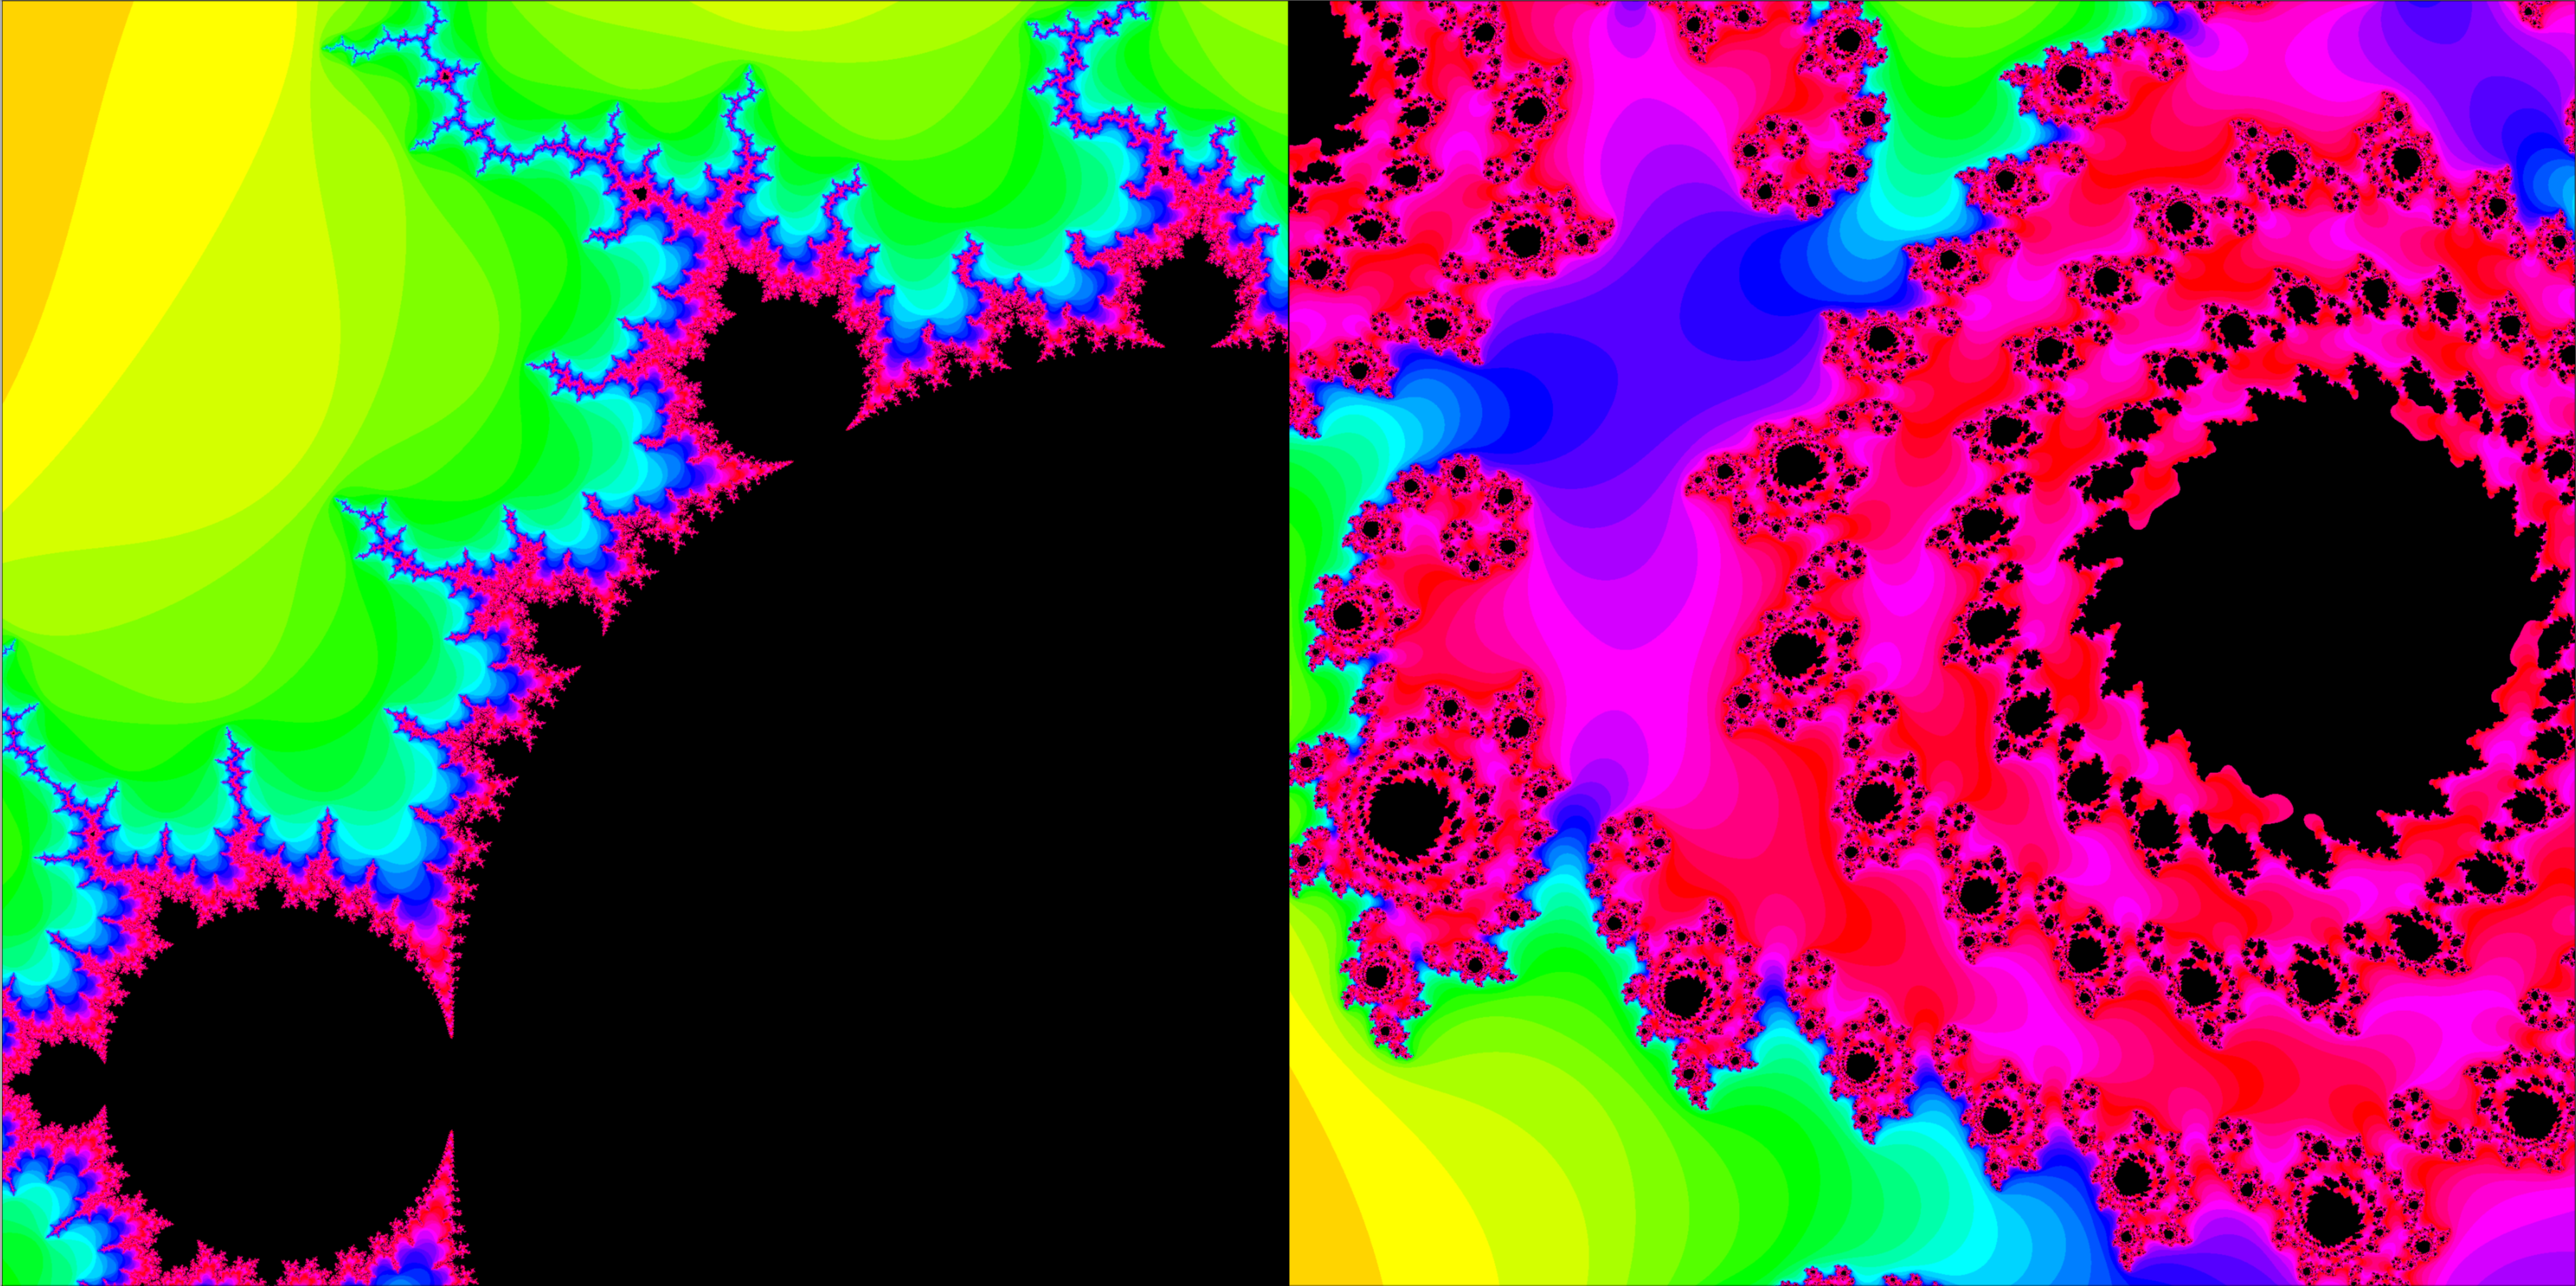
\includegraphics[width=\textwidth]{images/both.png}
\caption{This is a signle image showing the layout on the website, Mandelbrot on the left, Julia o nthe right}
\end{figure}

\paragraph{Real-Time Animations} 
Dynamic animations show the Julia set morphing in real time as different points within the Mandelbrot set are selected. This illustrates how varying complex constants impact the Julia set’s structure, giving users an intuitive understanding of the link between the two fractals. This cant be correctly shown in a PDF so either go to the Interactive Web View or See ZIP file for animations and videos.

\begin{figure}[H]
    \centering
    \subfloat[\centering Julia Set 1]{{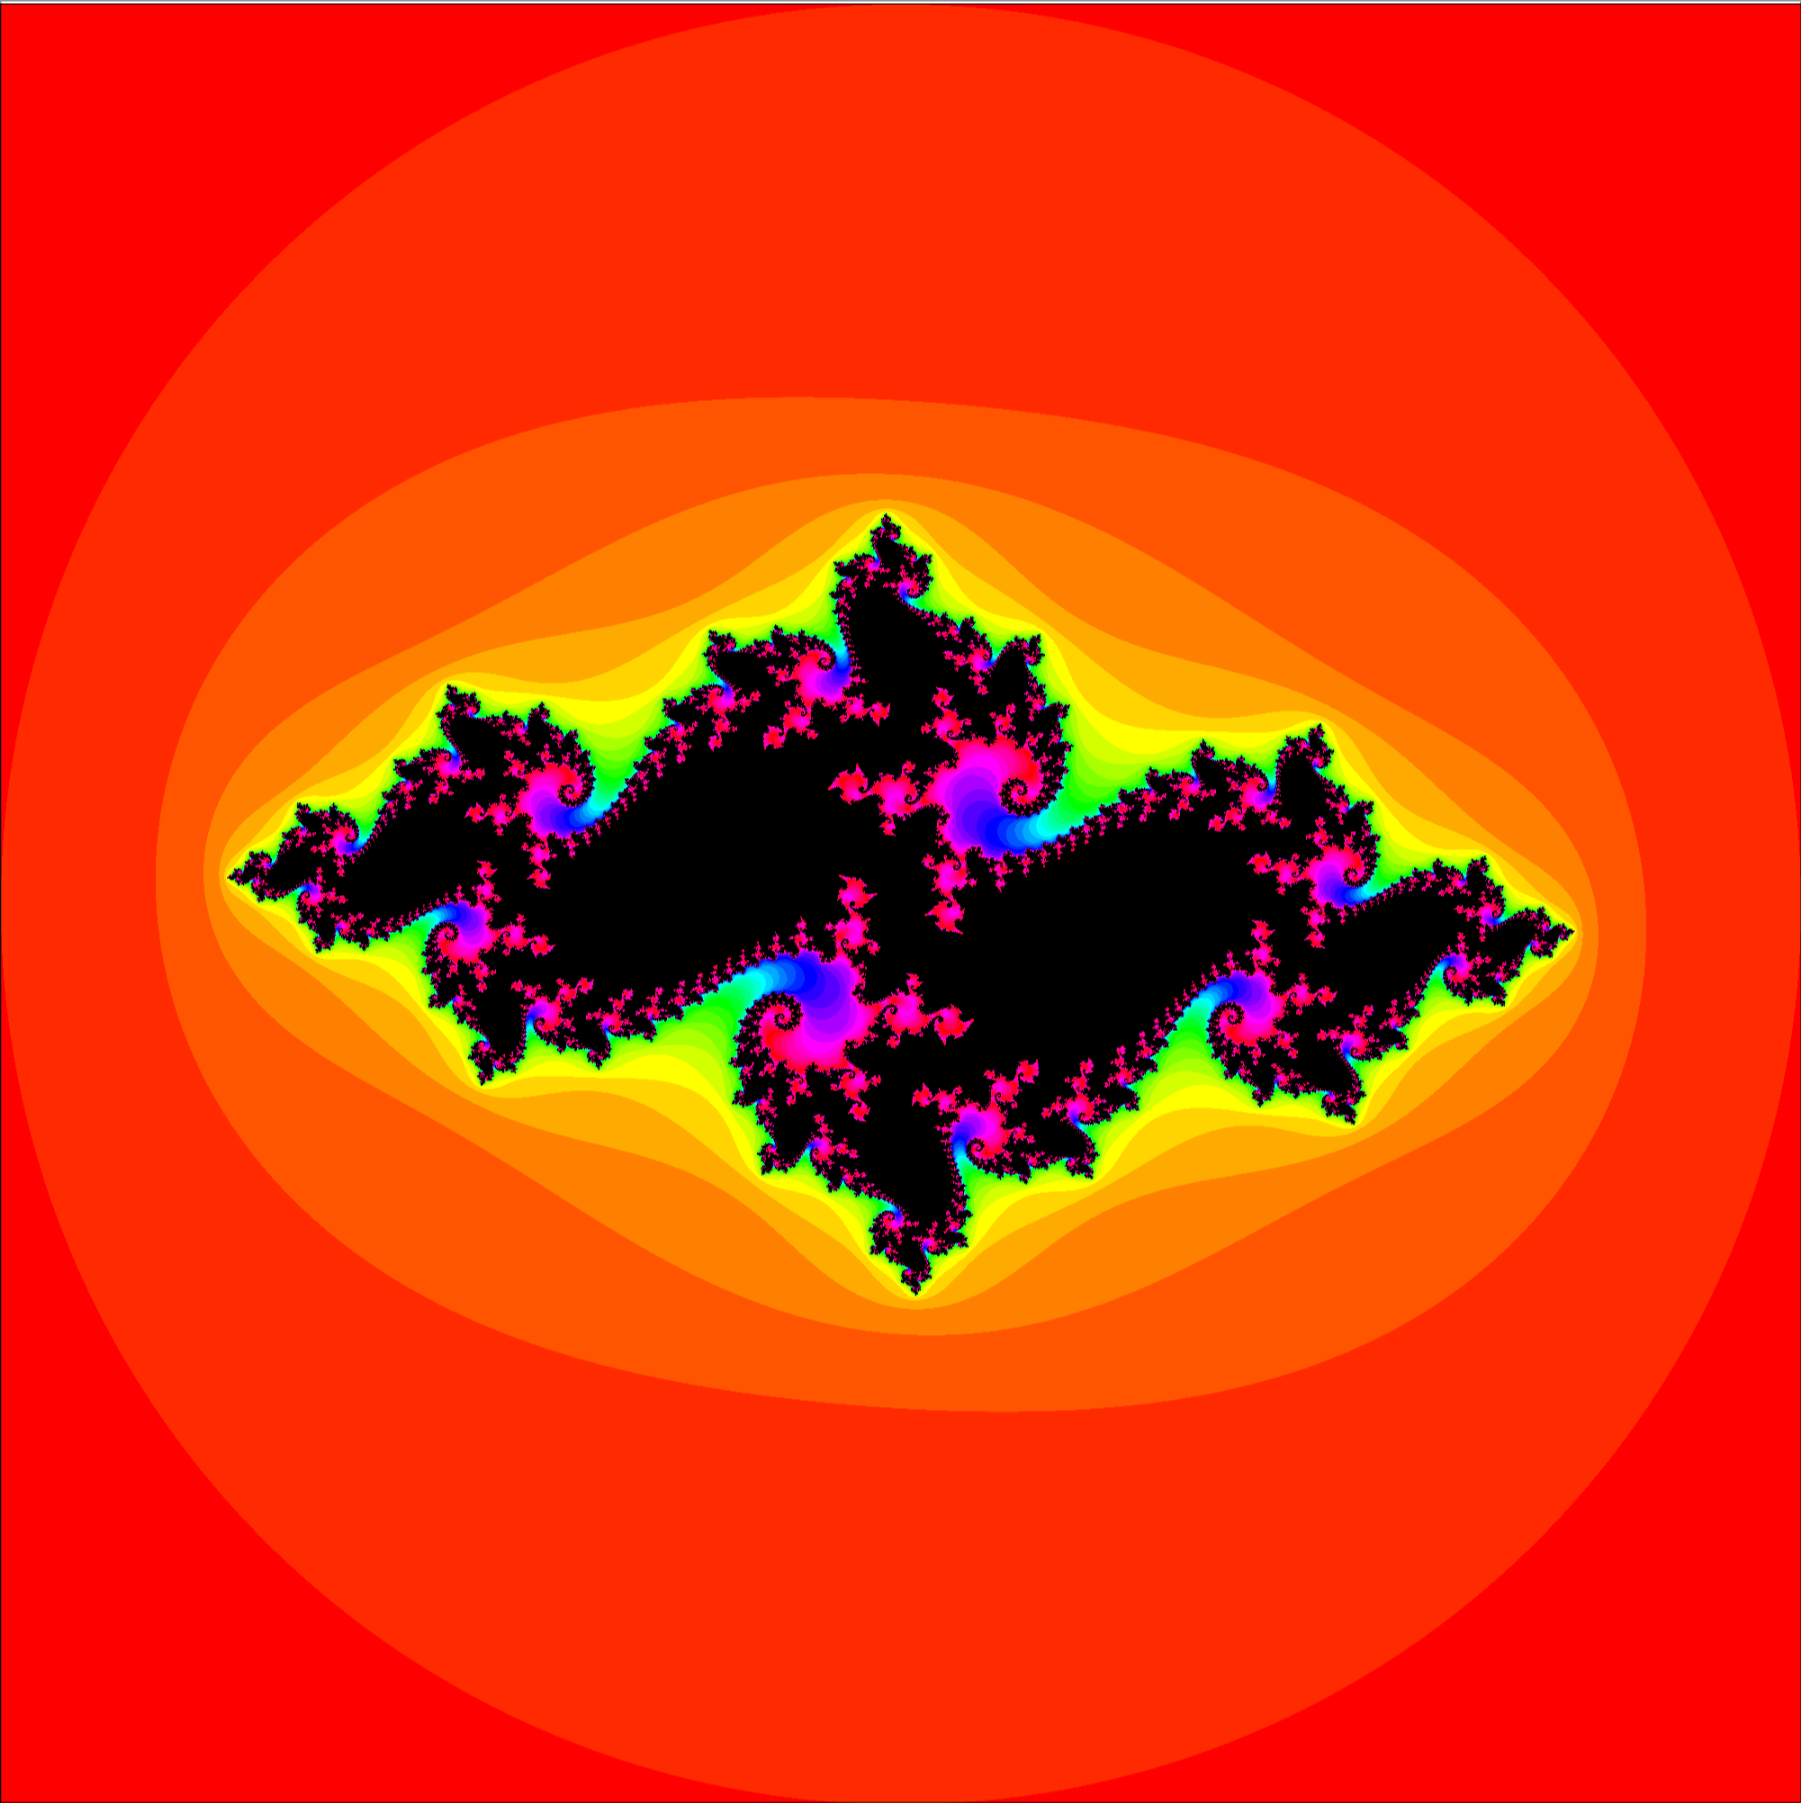
\includegraphics[width=0.4\textwidth]{images/julia set 1.png} }}%
    \qquad
    \subfloat[\centering Julia Set 1]{{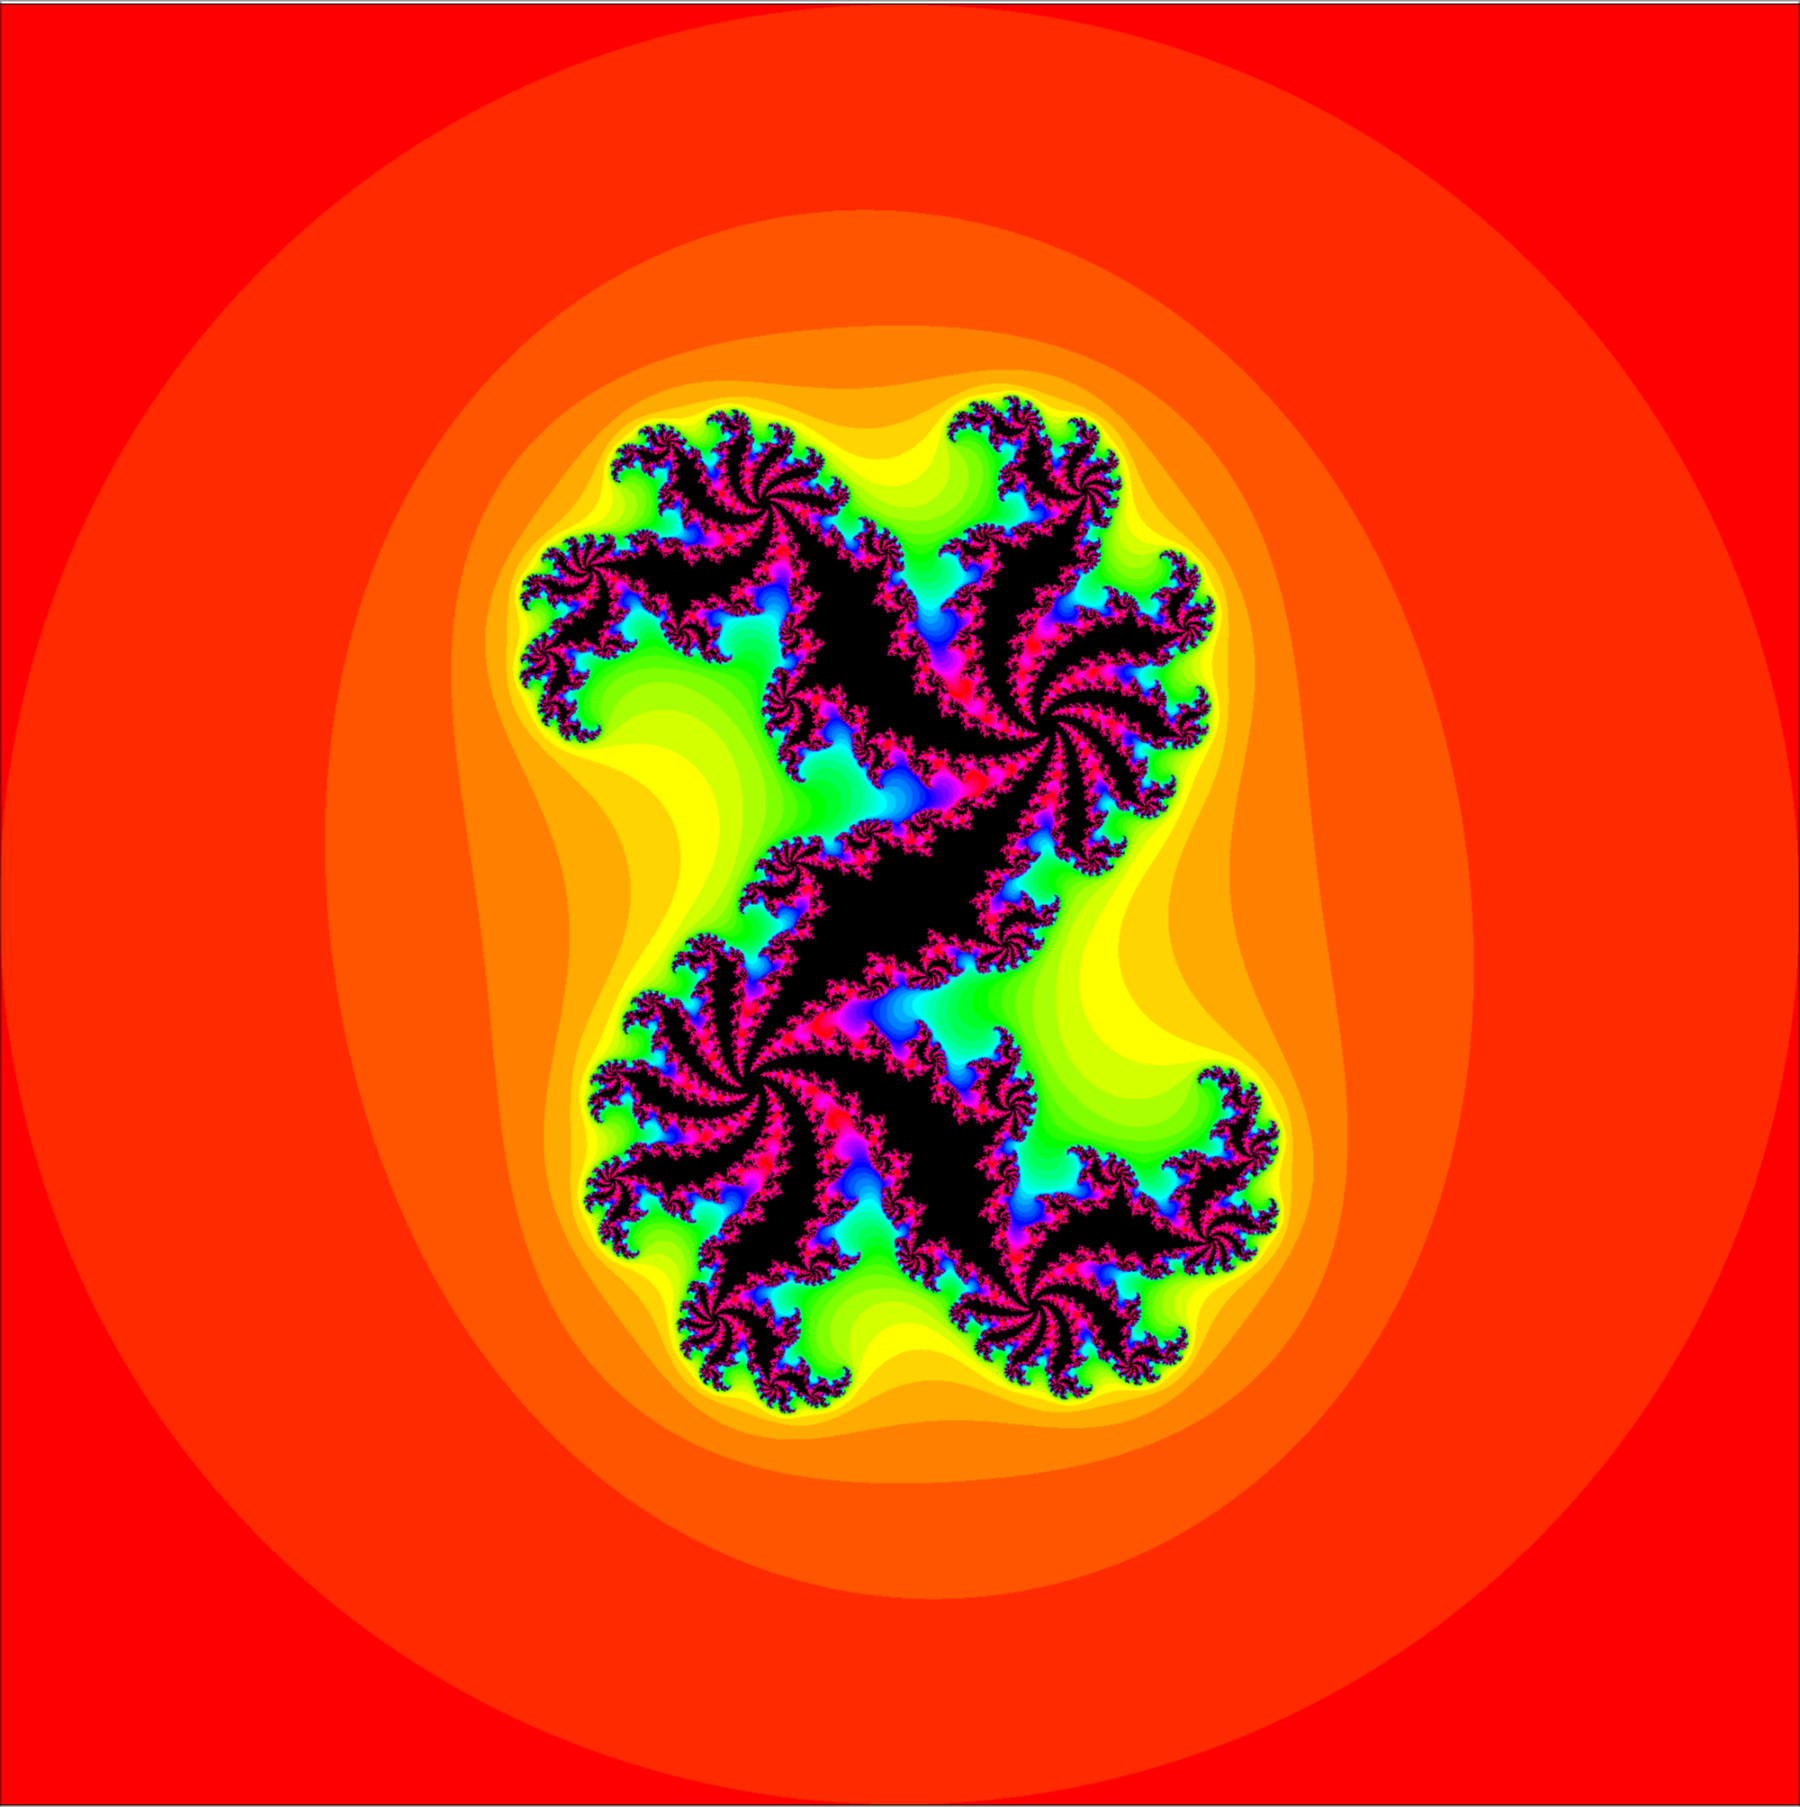
\includegraphics[width=0.4\textwidth]{images/julia set 2.png} }}%
    \caption{2 Julia Set Fractels with diffrent $C$ values}%
    \label{fig:example}%
\end{figure}

\begin{figure}[H]
\centering

\end{figure}

\paragraph{Interactive Zoom and Pan} 
An “infinite zoom” feature with adaptive resolution allows users to delve into fractal depths seamlessly. This zoom function displays finer details at each level, revealing recursive patterns and self-similarity within both fractals. This cant be correctly shown in a PDF so either go to the Interactive Web View or See ZIP file for animations and videos.

\begin{figure}[H]
\centering
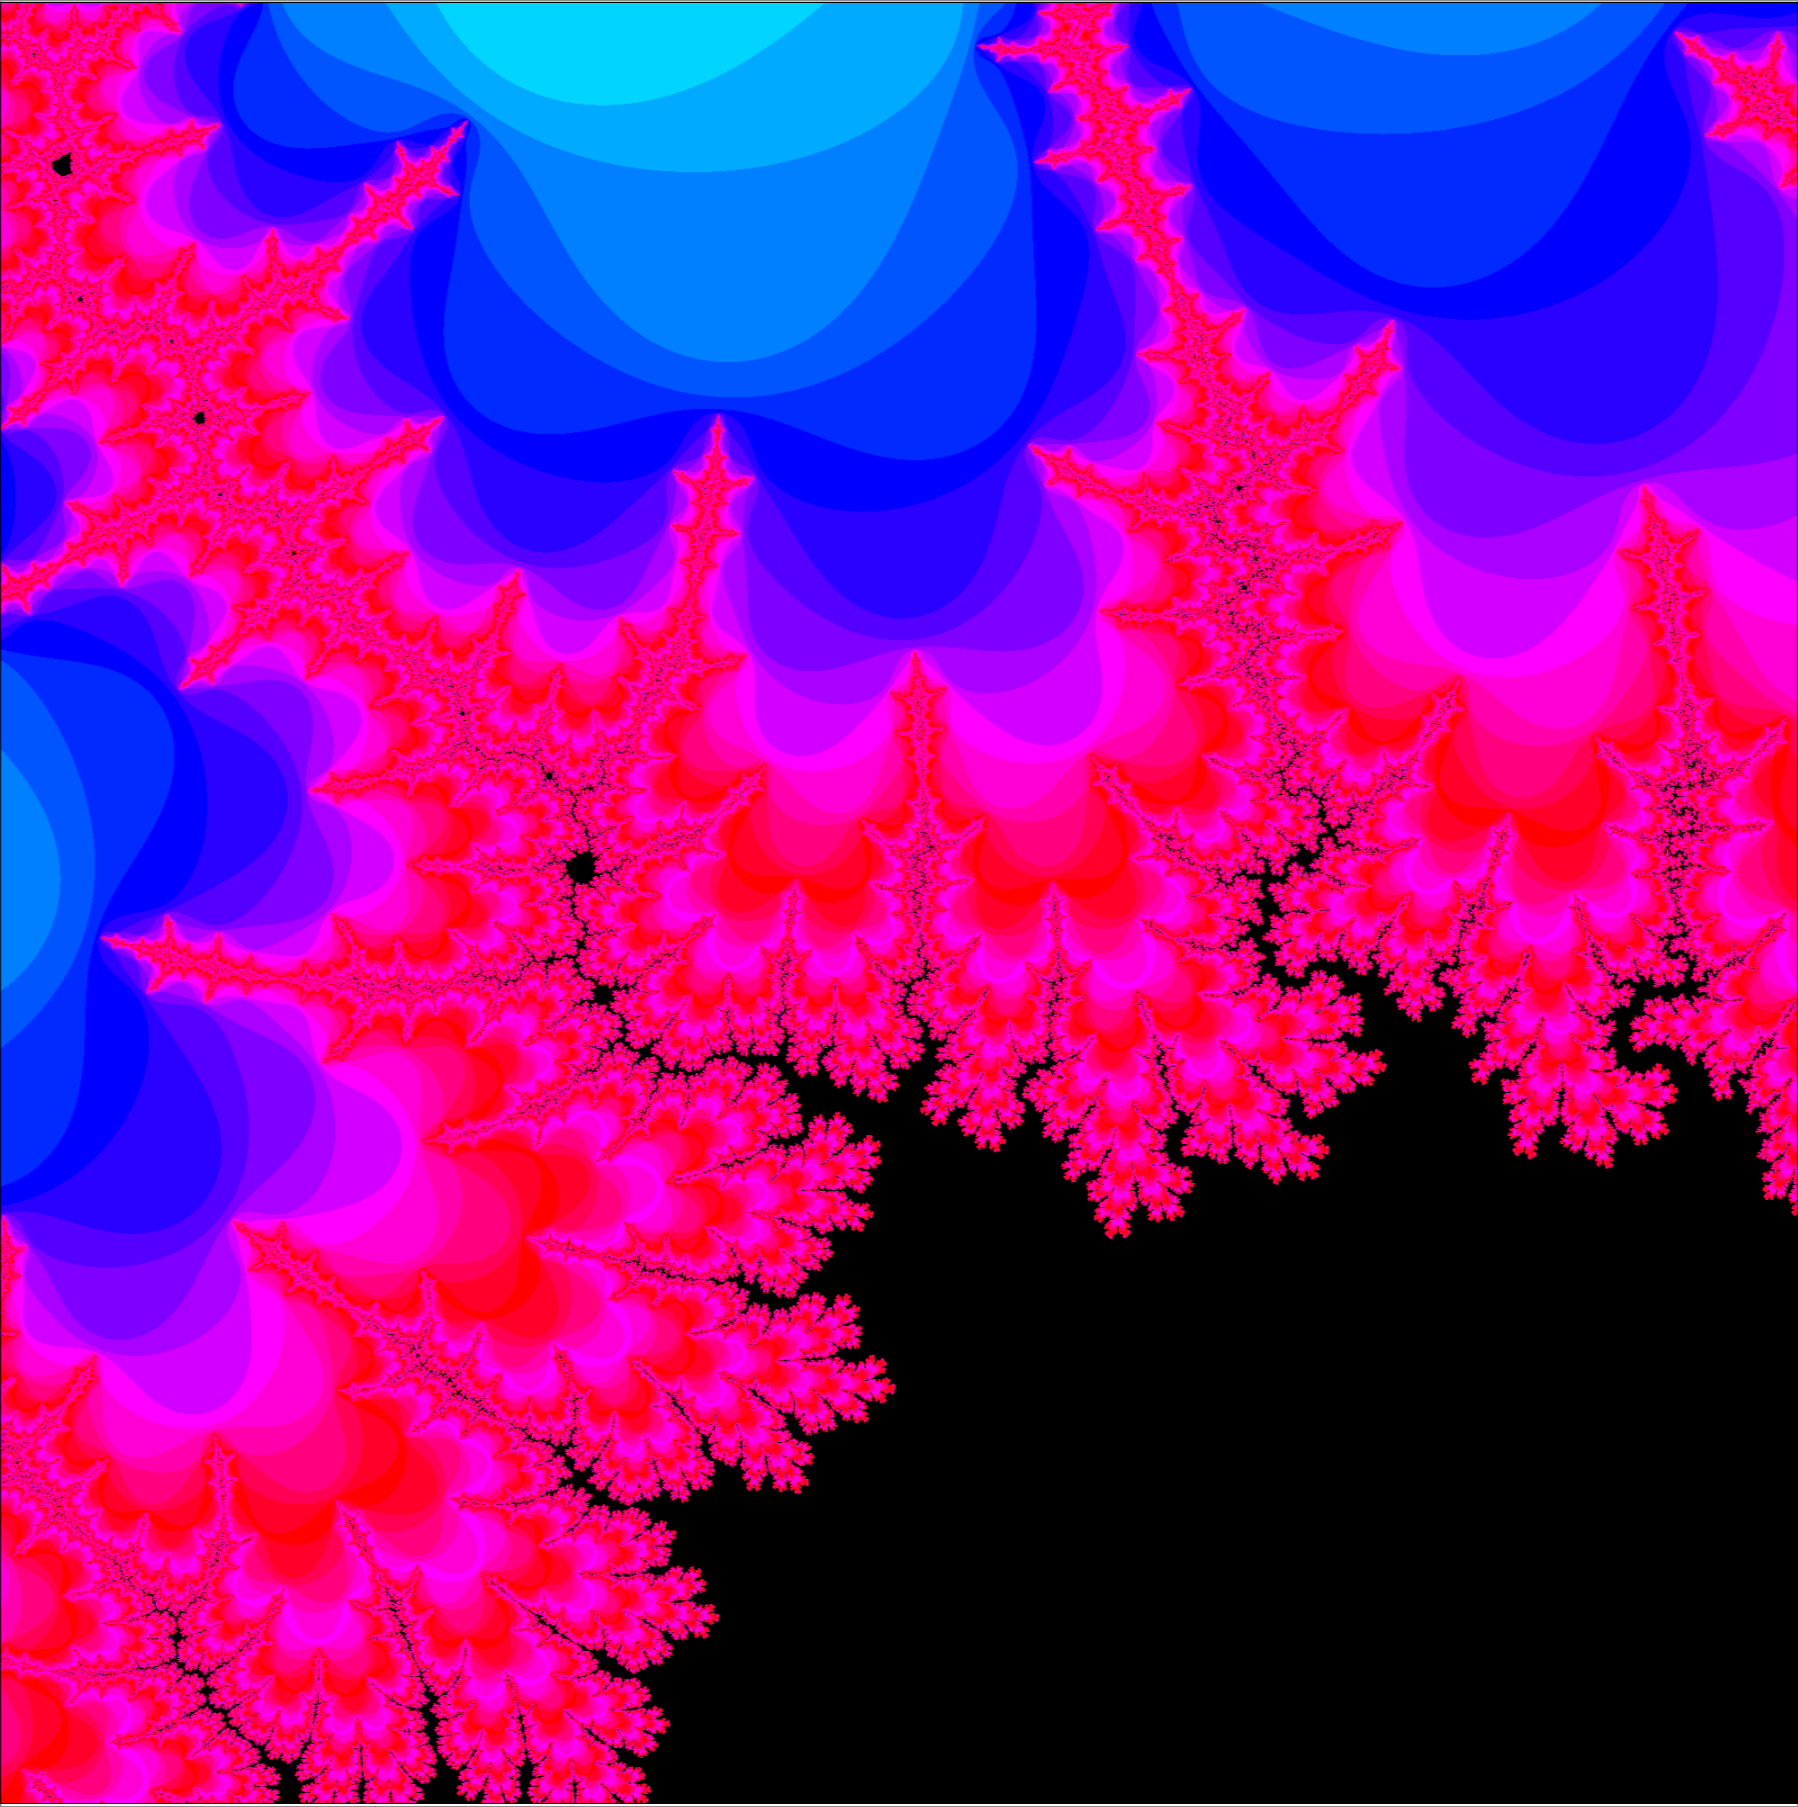
\includegraphics[width=\textwidth]{images/zoom.png}
\caption{Zoomed in area on the upper left central bulb}
\end{figure}

\subsection{Effective Visualisation issues}
To create effective fractal Visualisations, smooth gradient coloring was implemented to reveal escape times with seamless transitions across fractal boundaries. By interpolating colors based on partial escape times, the Visualisation minimized pixelation and visual noise, helping users distinguish the intricate details of stable and chaotic regions. This approach gave the fractal boundaries a cohesive, flowing appearance, which is especially valuable when exploring deeper levels of the fractal where fine distinctions are critical. 
\\\\
Adaptive resolution was also essential for enabling an “infinite zoom” feature, where detail recalculates dynamically at each zoom level. This technique allowed the fractal to retain sharp, high-resolution details during deep zooms without overwhelming processing resources. As users zoom closer, the fractal data is recalculated at higher precision, maintaining both visual clarity and performance. By focusing computational power on the areas where users are zoomed in, adaptive resolution preserved a fluid, lag-free experience, highlighting the fractal’s self-similar, recursive nature. 
\\\\
The real-time generation of the Julia set, triggered by selecting points within the Mandelbrot set, provided a highly interactive way to explore the relationship between these fractals. As users clicked or hovered over Mandelbrot points, the Julia set updated instantaneously, showing how different complex constants shape the Julia set’s structure. This interactivity gave users immediate visual feedback, making it easier to grasp complex mathematical relationships through direct exploration and observation. 
\\\\
Additionally, user-friendly controls for zoom, pan, and point selection made navigating the fractal space intuitive and engaging. The responsiveness of these features sustained user engagement and enabled a natural exploration of the fractals. Together, these Visualisation strategies improved the clarity, responsiveness, and educational effectiveness of the fractal Visualisations, making the complex nature of fractal geometry both accessible and captivating. 

\subsection{Insights and knowledge gained}
This project provided insights into fractal geometry, GPU-based rendering, and the power of interactivity in visual learning. Exploring the Mandelbrot and Julia sets deepened my understanding of fractal behavior, particularly how simple iterative formulas can generate complex, self-similar structures. Implementing fragment shaders in WebGL and optimizing with adaptive resolution taught me how to achieve real-time responsiveness without sacrificing detail, an approach valuable for future high-performance Visualisations.
\\\\
Additionally, integrating real-time updates and intuitive controls demonstrated how interactivity enhances learning by making abstract mathematical concepts accessible. Allowing users to select Mandelbrot points and instantly see corresponding Julia sets transformed complex relationships into an engaging, hands-on experience. This project reinforced the potential of interactive design for educational and exploratory Visualisation. 

\section{Exegesis of the Effectiveness of Visualisation Outputs}
The Visualisation outputs in this project were designed following principles of effective Visualisation to make complex fractal structures accessible and engaging. Each Visualisation output, as exemplified by all the fractal images in this report, was tailored to emphasize clarity, structure, and interactivity, allowing users to intuitively explore and understand fractal geometry.

\paragraph{Color Mapping and Contrast} 
Color is a central component in these Visualisations. High-contrast color gradients are applied to differentiate areas of stability (black regions) from chaotic areas that rapidly diverge. Warm colors, such as red and yellow, indicate higher escape velocities, while cooler colors (green and blue) are used for slower escape regions. This color scheme aligns with effective Visualisation practices by making regions of different behaviors easily distinguishable, allowing users to instantly recognize stability boundaries and transition zones within the fractal. 

\paragraph{Smooth Gradient Transitions}
Smooth gradients are used to avoid harsh transitions or pixelation, creating a continuous and visually appealing boundary between stable and chaotic regions. This approach is guided by the principle of reducing visual noise, as it minimizes abrupt color changes that might detract from the fractal’s structural detail. The gradient shading applied here helps users to see the fractal patterns clearly, enhancing the Visualisation’s readability and effectiveness.

\paragraph{Focus on Structure and Detail}
The fractal structures within the Mandelbrot and Julia sets are intricate and recursive, which can be challenging to visualise effectively. By focusing on high-resolution rendering, especially at deeper zoom levels, these Visualisations capture the fine details and self-similar patterns characteristic of fractals. Each level of zoom provides new layers of detail, helping to reveal the recursive nature of fractals in a way that supports exploratory learning. 

\paragraph{Responsive Interactivity}
While not visible in the static image, the interactive elements of these Visualisations are crucial for effective exploration. Features such as real-time Julia set updates and infinite zoom allow users to actively engage with the fractal, directly observing how changing parameters influence the visual output. This interactivity aligns with effective Visualisation criteria by enhancing user engagement and providing an intuitive means of exploring complex mathematical relationships. 

\paragraph{Balanced Visual Complexity}
Fractal Visualisations can become overwhelming if overly complex color schemes or shapes are used. To address this, the Visualisations maintain a balance, using vibrant colors in the chaotic regions while keeping stable regions in solid black, providing a sense of order amidst the complexity. This balance prevents cognitive overload, making the images aesthetically pleasing and scientifically insightful without overwhelming the viewer. 
\\\\
By following these design principles, the project effectively transforms complex fractal mathematics into accessible and engaging visual outputs that cater to both aesthetic appeal and educational value. These Visualisations make abstract mathematical concepts tangible, supporting users in exploring and understanding the intricate world of fractals. 

\section{Update Tasks and Project Timeline}

\subsection{Final Project Gant Chart}
\begin{figure}[H]
\centering
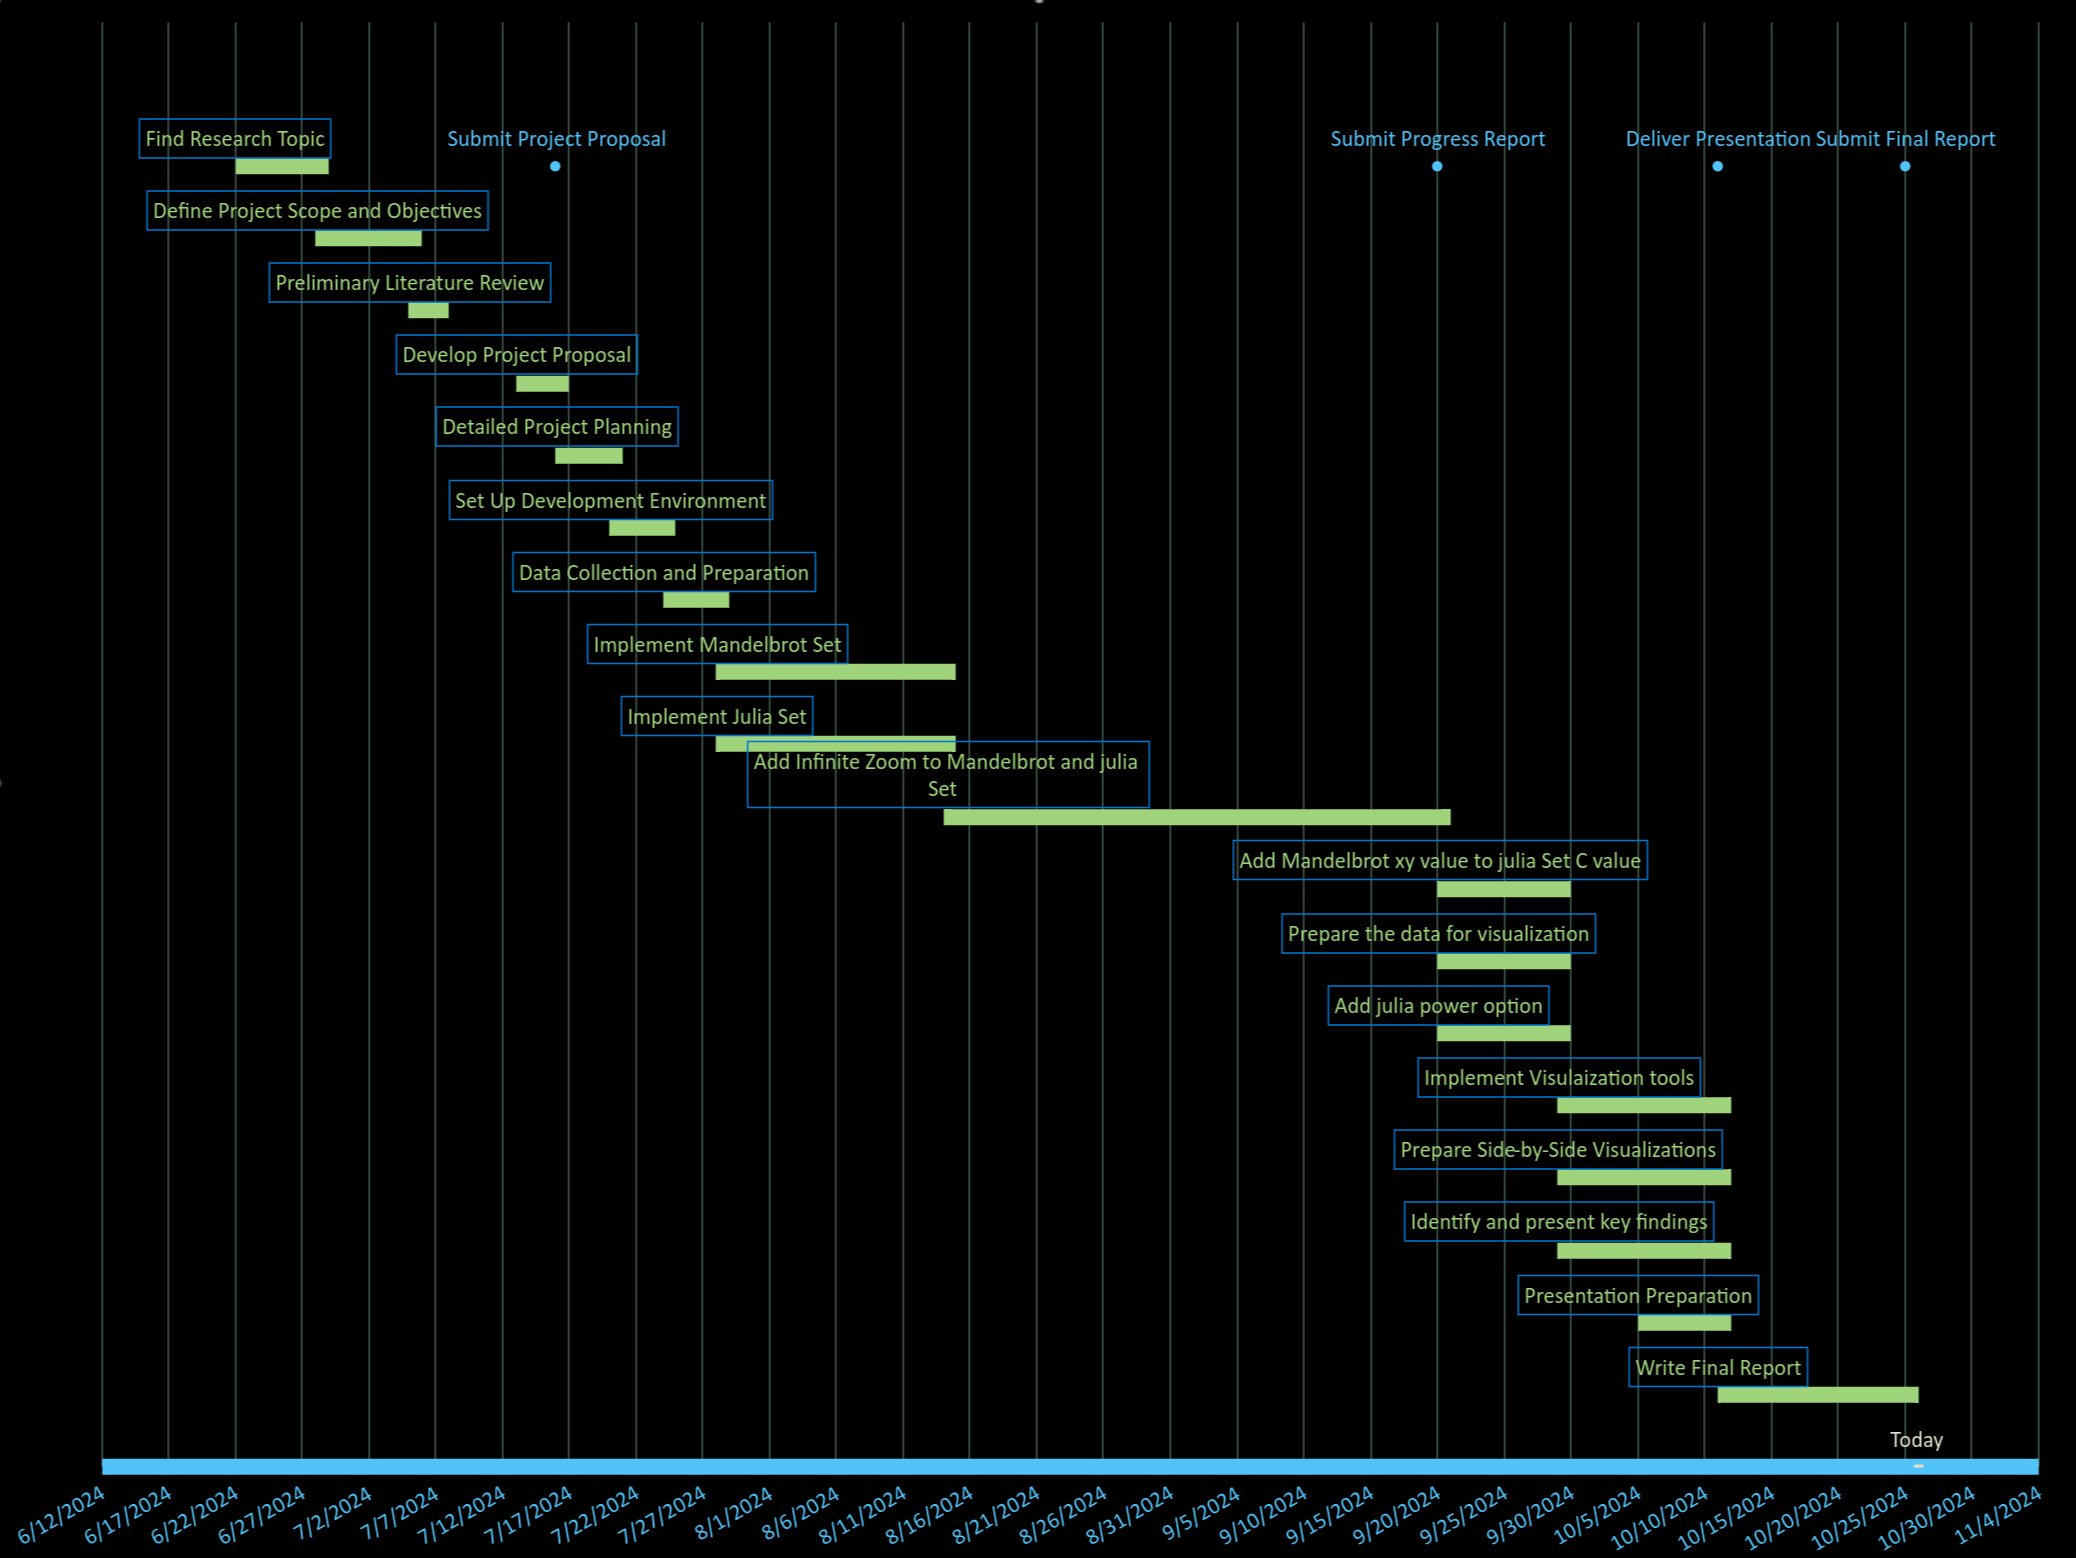
\includegraphics[width=\textwidth]{images/project gant chart.png}
\end{figure}

\section{Problems}
This project encountered several challenges, particularly with performance optimization, colour mapping, interactivity, and user interface design. 

\paragraph{Performance with Deep Zooming}
Infinite zooming was computationally demanding, often causing lag or browser crashes at high magnification. Adaptive resolution techniques helped optimize performance by recalculating fractal data based on zoom level, but balancing detail and fluidity remained challenging. Server-side rendering could be a future enhancement. 

\paragraph{Colour Mapping for Clarity}
Initially, colour schemes didn’t adequately highlight fractal boundaries, making distinctions between stable and chaotic regions unclear. Experimenting with smooth gradients ultimately provided the necessary clarity, emphasizing the impact of colour choices on visualization readability. 

\paragraph{Real-Time Interactivity}
Ensuring real-time Julia set updates for Mandelbrot selections required optimizing WebGL fragment shaders to minimize latency. This underscored the importance of efficient GPU-based computations and memory management in interactive visualizations. 

\paragraph{Edge Cases in Julia Sets}
Some Mandelbrot points generated Julia sets with minimal detail, reducing visual engagement. Adjusting iteration counts and escape conditions improved the results, highlighting the need for adaptable parameters in fractal algorithms.

\paragraph{User Interface Limitations}
Adding features like tooltips or preset zoom levels late in the project proved difficult. Prioritizing UI enhancements earlier would have improved user experience and engagement. 

\section{Project Journal}
\newpage


\section{Conclusion}
This project successfully developed an interactive visualization tool that explores the intricate relationships between the Mandelbrot and Julia sets. By leveraging WebGL and adaptive resolution, the tool achieved real-time rendering, smooth zooming, and responsive interactivity, allowing users to intuitively explore fractal geometry. The combination of smooth color gradients, infinite zoom, and real-time Julia set updates transformed complex mathematical concepts into accessible, engaging visuals, offering both educational and exploratory value. 
\\\\
Reflecting on the project, several aspects worked particularly well. The use of adaptive resolution was key to balancing performance and detail, enabling high-quality visuals without significant lag during deep zooming. Additionally, implementing smooth gradient shading greatly enhanced the visualization's readability, highlighting the fractal’s intricate boundaries and transitions. Interactivity, especially the real-time Julia set generation based on Mandelbrot point selection, provided an intuitive way for users to grasp the link between the two fractals. 
\\\\
However, there were also areas for improvement. Initially, color mapping and UI design were not fully optimized, impacting early usability and clarity. Prioritizing these elements earlier would have improved the user experience from the start. The challenges of implementing responsive interactivity and handling edge cases in Julia set generation emphasized the importance of algorithm flexibility and efficient memory management, lessons that would guide future projects. 
\\\\
For future work, expanding the visualization to include 3D fractals, such as the Mandelbulb, would offer a richer experience and provide a more immersive understanding of fractal geometry. Additionally, server-side rendering could enhance performance at extreme zoom levels, enabling even deeper fractal exploration without taxing client resources. UI enhancements, such as tooltips, guided tours, and preset zoom levels, could further improve usability, making the tool more intuitive for educational purposes. 
\\\\
In conclusion, this project demonstrated how interactive visualization can make abstract mathematical concepts accessible and engaging. The experience underscored the importance of balancing performance with visual detail and usability, laying a strong foundation for future exploration into real-time visualizations of complex data. 

\section{References}
\newpage


\section{Appendices}


\subsection{Code for Interactive Web interface (Javascript, WebGL)}

\begin{verbatim}
<!DOCTYPE html>
<html lang="en">
<head>
  <meta charset="UTF-8">
  <meta name="viewport" content="width=device-width, initial-scale=1.0">
  <title>Mandelbrot and Julia Sets</title>
  <style>
    canvas {
      border: 1px solid black;
    }
    #container {
      display: flex;
    }
  </style>
</head>
<body>
  <div style="display: flex; font-size: xx-large;">
    <div style="padding: 10px; width: 50%;">
      <h2 id="xyValue"></h2>
      <h2 id="cValue"></h2>
      <button id="resetZoomButton"><h1>Reset</h1></button>
  
      <label for="juliaPower">Julia Set Power</label>
      <input type="range" id="juliaPower" min="2" max="10" step="1" value="2">
      <label id="juliaPowerNumber">2</label>
      
      <button id="mandelbrotImage"><h1>Get Mandelbrot Image</h1></button>

      <button id="juliaImage"><h1>Julia Image</h1></button>
    </div>
    <div style="width: 50%;">
      <h2>Controls:</h2>
      <p>
        <b>Change scale of browser to fit canvases</b>
        <br>
        Mandelbrot Set left, Julia Set Right
        <br>
        Zoom: Mouse wheel (Both Fractals)
        <br>
        Selecting C value in Mandelbrot Set: Left Click and drag 
        (Can hold left click and drag around for real time changes)
      </p>
    </div>

  </div>

  <div id="container">
    <canvas id="mandelbrot" width="2000" height="2000"></canvas>
    <canvas id="julia" width="2000" height="2000"></canvas>
  </div>
  <script type="module">
    const mandelbrotCanvas = document.getElementById('mandelbrot');
    const juliaCanvas = document.getElementById('julia');

    const glMandelbrot = mandelbrotCanvas.getContext('webgl', 
    { preserveDrawingBuffer: true });
    const ctxMandelbrot = mandelbrotCanvas.getContext('2d');
    
    const glJulia = juliaCanvas.getContext('webgl', 
    { preserveDrawingBuffer: true });
    const ctxJulia = juliaCanvas.getContext('2d');


    const cValue = document.getElementById("cValue")
    const xyValue = document.getElementById("xyValue")
    const juliaPowerSlider = document.getElementById('juliaPower');
    const juliaPowerNumber = document.getElementById("juliaPowerNumber")

    const mandelbrotImage = document.getElementById("mandelbrotImage");
    const juliaImage = document.getElementById("juliaImage");

    let cr = 0;
    let ci = 0;
    let juliaPower = 2;

    const maxIterations = 100;
    let mandelbrotZoom = { xMin: -2, xMax: 2, yMin: -2, yMax: 2 };
    let juliaZoom = { xMin: -2, xMax: 2, yMin: -2, yMax: 2 };

    function createShader(gl, type, source) {
      const shader = gl.createShader(type);
      gl.shaderSource(shader, source);
      gl.compileShader(shader);
      if (!gl.getShaderParameter(shader, gl.COMPILE_STATUS)) {
        console.error('An error occurred compiling the shaders: ' 
        + gl.getShaderInfoLog(shader));
        gl.deleteShader(shader);
        return null;
      }
      return shader;
    }

    function createProgram(gl, vertexShader, fragmentShader) {
      const program = gl.createProgram();
      gl.attachShader(program, vertexShader);
      gl.attachShader(program, fragmentShader);
      gl.linkProgram(program);
      if (!gl.getProgramParameter(program, gl.LINK_STATUS)) {
        console.error('Unable to initialize the shader program: ' 
        + gl.getProgramInfoLog(program));
        return null;
      }
      return program;
    }

    function drawMandelbrot() {
      const width = mandelbrotCanvas.width;
      const height = mandelbrotCanvas.height;

      const vertexShaderSource = `
        attribute vec4 position;
        void main() {
          gl_Position = position;
        }
      `;

      const fragmentShaderSource = `
        precision highp float;
        uniform float xMin;
        uniform float xMax;
        uniform float yMin;
        uniform float yMax;
        uniform float maxIterations;
        void main() {
          float cr = xMin + (gl_FragCoord.x / ${width}.0) * (xMax - xMin);
          float ci = yMin + (gl_FragCoord.y / ${height}.0) * (yMax - yMin);
          float zr = 0.0;
          float zi = 0.0;
          float iteration = 0.0;

          for (int i = 0; i < 1000; i++) {
            if (zr * zr + zi * zi >= 4.0 || iteration >= maxIterations) {
              break;
            }
            float tmp = zr * zr - zi * zi + cr;
            zi = 2.0 * zr * zi + ci;
            zr = tmp;
            iteration++;
          }

          if (iteration == maxIterations) {
            gl_FragColor = vec4(0, 0, 0, 0);
          } else {
            float hue = iteration * 10.0;
            float saturation = 1.0;
            float lightness = 0.5;
            float c = (1.0 - abs(2.0 * lightness - 1.0)) * saturation;
            float x = c * (1.0 - abs(mod(hue / 60.0, 2.0) - 1.0));
            float m = lightness - c / 2.0;
            vec3 rgb;

            if (hue < 60.0) {
              rgb = vec3(c, x, 0.0);
            } else if (hue < 120.0) {
              rgb = vec3(x, c, 0.0);
            } else if (hue < 180.0) {
              rgb = vec3(0.0, c, x);
            } else if (hue < 240.0) {
              rgb = vec3(0.0, x, c);
            } else if (hue < 300.0) {
              rgb = vec3(x, 0.0, c);
            } else {
              rgb = vec3(c, 0.0, x);
            }

            gl_FragColor = vec4(rgb + vec3(m), 1.0);
          }
        }
      `;

      const vertexShader = createShader(glMandelbrot, 
      glMandelbrot.VERTEX_SHADER, vertexShaderSource);
      const fragmentShader = createShader(glMandelbrot, 
      glMandelbrot.FRAGMENT_SHADER, fragmentShaderSource);
      const program = createProgram(glMandelbrot, 
      vertexShader, fragmentShader);

      const positionAttributeLocation = glMandelbrot
      .getAttribLocation(program, 'position');
      const positionBuffer = glMandelbrot.createBuffer();
      glMandelbrot.bindBuffer(glMandelbrot.ARRAY_BUFFER, 
      positionBuffer);
      glMandelbrot.bufferData(glMandelbrot.ARRAY_BUFFER, 
      new Float32Array([
        -1, -1,
         1, -1,
        -1,  1,
        -1,  1,
         1, -1,
         1,  1,
      ]), glMandelbrot.STATIC_DRAW);

      glMandelbrot.viewport(0, 0, width, height);
      glMandelbrot.clearColor(0, 0, 0, 0);
      glMandelbrot.clear(glMandelbrot.COLOR_BUFFER_BIT);

      glMandelbrot.useProgram(program);

      glMandelbrot.enableVertexAttribArray(
      positionAttributeLocation);
      glMandelbrot.bindBuffer(glMandelbrot.ARRAY_BUFFER, 
      positionBuffer);
      glMandelbrot.vertexAttribPointer(positionAttributeLocation, 
      2, glMandelbrot.FLOAT, false, 0, 0);

      glMandelbrot.uniform1f(glMandelbrot.getUniformLocation(
      program, 'xMin'), mandelbrotZoom.xMin);
      glMandelbrot.uniform1f(glMandelbrot.getUniformLocation(
      program, 'xMax'), mandelbrotZoom.xMax);
      glMandelbrot.uniform1f(glMandelbrot.getUniformLocation(
      program, 'yMin'), mandelbrotZoom.yMax);
      glMandelbrot.uniform1f(glMandelbrot.getUniformLocation(
      program, 'yMax'), mandelbrotZoom.yMin);

      glMandelbrot.uniform1f(glMandelbrot.getUniformLocation(
      program, 'maxIterations'), maxIterations);

      glMandelbrot.drawArrays(glMandelbrot.TRIANGLES, 0, 6);

      // Draw dot where cr, ci are located using WebGL
      const dotVertexShaderSource = `
        attribute vec4 position;
        void main() {
          gl_PointSize = 10.0;
          gl_Position = position;
        }
      `;

      const dotFragmentShaderSource = `
        precision highp float;
        void main() {
          gl_FragColor = vec4(1.0, 0.0, 0.0, 1.0); // Red color
        }
      `;

      const dotVertexShader = createShader(glMandelbrot, 
      glMandelbrot.VERTEX_SHADER, dotVertexShaderSource);
      const dotFragmentShader = createShader(glMandelbrot, 
      glMandelbrot.FRAGMENT_SHADER, dotFragmentShaderSource);
      const dotProgram = createProgram(glMandelbrot, 
      dotVertexShader, dotFragmentShader);

      const dotPositionAttributeLocation = glMandelbrot
      .getAttribLocation(dotProgram, 'position');
      const dotPositionBuffer = glMandelbrot.createBuffer();
      glMandelbrot.bindBuffer(glMandelbrot.ARRAY_BUFFER, 
      dotPositionBuffer);

      // const cr = (mandelbrotZoom.xMin + 
      mandelbrotZoom.xMax) / 2.0;
      // const ci = (mandelbrotZoom.yMin + 
      mandelbrotZoom.yMax) / 2.0;
      const dotX = (cr - mandelbrotZoom.xMin) / 
      (mandelbrotZoom.xMax - mandelbrotZoom.xMin) * 2.0 - 1.0;
      const dotY = (ci - mandelbrotZoom.yMin) / 
      (mandelbrotZoom.yMax - mandelbrotZoom.yMin) * 2.0 - 1.0;

      glMandelbrot.bufferData(glMandelbrot.ARRAY_BUFFER, 
      new Float32Array([dotX, dotY * -1]), glMandelbrot.STATIC_DRAW);

      glMandelbrot.useProgram(dotProgram);
      glMandelbrot.enableVertexAttribArray(dotPositionAttributeLocation);
      glMandelbrot.vertexAttribPointer(dotPositionAttributeLocation, 
      2, glMandelbrot.FLOAT, false, 0, 0);
      glMandelbrot.drawArrays(glMandelbrot.POINTS, 0, 1);
    }

    function drawJulia(cr, ci) {
      cValue.innerText = `Julia Set: c = ${cr} + ${ci}i`
      xyValue.innerText = `Mandelbrot Set location: x = ${cr}, y = ${ci}`
      const width = juliaCanvas.width;
      const height = juliaCanvas.height;

      const vertexShaderSource = `
        attribute vec4 position;
        void main() {
          gl_Position = position;
        }
      `;

      const fragmentShaderSource = `
        precision highp float;
        uniform float cr;
        uniform float ci;
        uniform float xMin;
        uniform float xMax;
        uniform float yMin;
        uniform float yMax;
        uniform float maxIterations;
        uniform float power;
        void main() {
          float zr = xMin + (gl_FragCoord.x / ${width}.0) * (xMax - xMin);
          float zi = yMin + (gl_FragCoord.y / ${height}.0) * (yMax - yMin);
          float iteration = 0.0;

          for (int i = 0; i < 1000; i++) {
            if (zr * zr + zi * zi >= 4.0 || iteration >= maxIterations) {
              break;
            }

            float r = pow(zr * zr + zi * zi, power / 2.0);
            float theta = atan(zi, zr) * power;
            zr = r * cos(theta) + cr;
            zi = r * sin(theta) + ci;
            iteration++;
          }

          if (iteration == maxIterations) {
            gl_FragColor = vec4(0, 0, 0, 0);
          } else {
            float hue = iteration * 10.0;
            float saturation = 1.0;
            float lightness = 0.5;
            float c = (1.0 - abs(2.0 * lightness - 1.0)) * saturation;
            float x = c * (1.0 - abs(mod(hue / 60.0, 2.0) - 1.0));
            float m = lightness - c / 2.0;
            vec3 rgb;

            if (hue < 60.0) {
              rgb = vec3(c, x, 0.0);
            } else if (hue < 120.0) {
              rgb = vec3(x, c, 0.0);
            } else if (hue < 180.0) {
              rgb = vec3(0.0, c, x);
            } else if (hue < 240.0) {
              rgb = vec3(0.0, x, c);
            } else if (hue < 300.0) {
              rgb = vec3(x, 0.0, c);
            } else {
              rgb = vec3(c, 0.0, x);
            }

            gl_FragColor = vec4(rgb + vec3(m), 1.0);
          }
        }
      `;

      const vertexShader = createShader(glJulia, 
      glJulia.VERTEX_SHADER, vertexShaderSource);
      const fragmentShader = createShader(glJulia, 
      glJulia.FRAGMENT_SHADER, fragmentShaderSource);
      const program = createProgram(glJulia, 
      vertexShader, fragmentShader);

      const positionAttributeLocation = glJulia.getAttribLocation(
      program, 'position');
      const positionBuffer = glJulia.createBuffer();
      glJulia.bindBuffer(glJulia.ARRAY_BUFFER, positionBuffer);
      glJulia.bufferData(glJulia.ARRAY_BUFFER, new Float32Array([
        -1, -1,
         1, -1,
        -1,  1,
        -1,  1,
         1, -1,
         1,  1,
      ]), glJulia.STATIC_DRAW);

      glJulia.viewport(0, 0, width, height);
      glJulia.clearColor(0, 0, 0, 0);
      glJulia.clear(glJulia.COLOR_BUFFER_BIT);

      glJulia.useProgram(program);

      glJulia.enableVertexAttribArray(positionAttributeLocation);
      glJulia.bindBuffer(glJulia.ARRAY_BUFFER, positionBuffer);
      glJulia.vertexAttribPointer(positionAttributeLocation, 2, 
      glJulia.FLOAT, false, 0, 0);

      glJulia.uniform1f(glJulia.getUniformLocation(program, 'cr'), 
      cr);
      glJulia.uniform1f(glJulia.getUniformLocation(program, 'ci'), 
      ci);

      glJulia.uniform1f(glJulia.getUniformLocation(program, 'xMin'), 
      juliaZoom.xMin);
      glJulia.uniform1f(glJulia.getUniformLocation(program, 'xMax'), 
      juliaZoom.xMax);
      glJulia.uniform1f(glJulia.getUniformLocation(program, 'yMin'), 
      juliaZoom.yMax);
      glJulia.uniform1f(glJulia.getUniformLocation(program, 'yMax'), 
      juliaZoom.yMin);

      glJulia.uniform1f(glJulia.getUniformLocation(program, 
      'maxIterations'), maxIterations);

      glJulia.uniform1f(glJulia.getUniformLocation(program, 
      'power'), juliaPower);

      glJulia.drawArrays(glJulia.TRIANGLES, 0, 6);
    }

    let buttonClick = false

    document.addEventListener("mousedown", (event) => {
      buttonClick = true
    });

    document.addEventListener("mouseup", (event) => {
      buttonClick = false
      drawMandelbrot();
    });

    mandelbrotCanvas.addEventListener('mousemove', (e) => {
      if (buttonClick) {
        const rect = mandelbrotCanvas.getBoundingClientRect();
        const mouseX = e.clientX - rect.left;
        const mouseY = e.clientY - rect.top;
        cr = mandelbrotZoom.xMin + (mouseX / mandelbrotCanvas.width) 
        * (mandelbrotZoom.xMax - mandelbrotZoom.xMin);
        ci = mandelbrotZoom.yMin + (mouseY / mandelbrotCanvas.height) 
        * (mandelbrotZoom.yMax - mandelbrotZoom.yMin);
        drawJulia(cr, ci);
      }

    });

    mandelbrotCanvas.addEventListener('wheel', (e) => {
      e.preventDefault();
      const zoomFactor = 0.9;
      const mouseX = e.offsetX;
      const mouseY = e.offsetY;
      const xCenter = mandelbrotZoom.xMin + (mouseX / mandelbrotCanvas.width) 
      * (mandelbrotZoom.xMax - mandelbrotZoom.xMin);
      const yCenter = mandelbrotZoom.yMin + (mouseY / mandelbrotCanvas.height) 
      * (mandelbrotZoom.yMax - mandelbrotZoom.yMin);

      if (e.deltaY < 0) {
        // Zoom in
        mandelbrotZoom.xMin = xCenter + (mandelbrotZoom.xMin - xCenter) 
        * zoomFactor;
        mandelbrotZoom.xMax = xCenter + (mandelbrotZoom.xMax - xCenter) 
        * zoomFactor;
        mandelbrotZoom.yMin = yCenter + (mandelbrotZoom.yMin - yCenter) 
        * zoomFactor;
        mandelbrotZoom.yMax = yCenter + (mandelbrotZoom.yMax - yCenter) 
        * zoomFactor;
      } else {
        // Zoom out
        mandelbrotZoom.xMin = xCenter + (mandelbrotZoom.xMin - xCenter) 
        / zoomFactor;
        mandelbrotZoom.xMax = xCenter + (mandelbrotZoom.xMax - xCenter) 
        / zoomFactor;
        mandelbrotZoom.yMin = yCenter + (mandelbrotZoom.yMin - yCenter) 
        / zoomFactor;
        mandelbrotZoom.yMax = yCenter + (mandelbrotZoom.yMax - yCenter) 
        / zoomFactor;
      }

      drawMandelbrot();
    });

    juliaCanvas.addEventListener('wheel', (e) => {
      e.preventDefault();
      const zoomFactor = 0.9;
      const mouseX = e.offsetX;
      const mouseY = e.offsetY;
      const xCenter = juliaZoom.xMin + (mouseX / juliaCanvas.width) 
      * (juliaZoom.xMax - juliaZoom.xMin);
      const yCenter = juliaZoom.yMin + (mouseY / juliaCanvas.height) 
      * (juliaZoom.yMax - juliaZoom.yMin);

      if (e.deltaY < 0) {
        // Zoom in
        juliaZoom.xMin = xCenter + (juliaZoom.xMin - xCenter) * zoomFactor;
        juliaZoom.xMax = xCenter + (juliaZoom.xMax - xCenter) * zoomFactor;
        juliaZoom.yMin = yCenter + (juliaZoom.yMin - yCenter) * zoomFactor;
        juliaZoom.yMax = yCenter + (juliaZoom.yMax - yCenter) * zoomFactor;
      } else {
        // Zoom out
        juliaZoom.xMin = xCenter + (juliaZoom.xMin - xCenter) / zoomFactor;
        juliaZoom.xMax = xCenter + (juliaZoom.xMax - xCenter) / zoomFactor;
        juliaZoom.yMin = yCenter + (juliaZoom.yMin - yCenter) / zoomFactor;
        juliaZoom.yMax = yCenter + (juliaZoom.yMax - yCenter) / zoomFactor;
      }

      drawJulia(cr, ci);
    });

    document.getElementById("resetZoomButton").addEventListener("click", (e) => {

      mandelbrotZoom = { xMin: -2, xMax: 2, yMin: -2, yMax: 2 };
      juliaZoom = { xMin: -2, xMax: 2, yMin: -2, yMax: 2 };
      juliaPower = 2

      drawMandelbrot();
      drawJulia(cr, ci);
    })

    juliaPowerSlider.addEventListener('input', (e) => {
      juliaPower = parseFloat(e.target.value);
      juliaPowerNumber.innerText = juliaPower
      drawJulia(cr, ci);
    });

    mandelbrotImage.addEventListener('click', (e) => {
      var MIME_TYPE = "image/png";

      var imgURL = mandelbrotCanvas.toDataURL(MIME_TYPE);

      var dlLink = document.createElement('a');
      dlLink.download = "mandelbrot_image.png";
      dlLink.href = imgURL;
      dlLink.dataset.downloadurl = [MIME_TYPE, dlLink.download, 
      dlLink.href].join(':');

      document.body.appendChild(dlLink);
      dlLink.click();
      document.body.removeChild(dlLink);
    })

    juliaImage.addEventListener('click', (e) => {
      var MIME_TYPE = "image/png";

      var imgURL = juliaCanvas.toDataURL(MIME_TYPE);

      var dlLink = document.createElement('a');
      dlLink.download = "julia_image.png";
      dlLink.href = imgURL;
      dlLink.dataset.downloadurl = [MIME_TYPE, dlLink.download, 
      dlLink.href].join(':');

      document.body.appendChild(dlLink);
      dlLink.click();
      document.body.removeChild(dlLink);
    })

    drawMandelbrot();
    drawJulia(0, 0);
  </script>
</body>
</html>
\end{verbatim}






\end{document}